\documentclass[11pt]{article}
\usepackage[utf8]{inputenc}
\usepackage{amsmath}
\usepackage{amssymb}
\usepackage{color, soul}
\usepackage[usenames,dvipsnames]{xcolor}
\usepackage{tikz}
\usetikzlibrary{arrows}
\tikzset{
    vertex/.style={
        circle,fill=black,scale=0.5
        },
    blank/.style={
        circle,fill=white
        },
    }

\begin{document}

    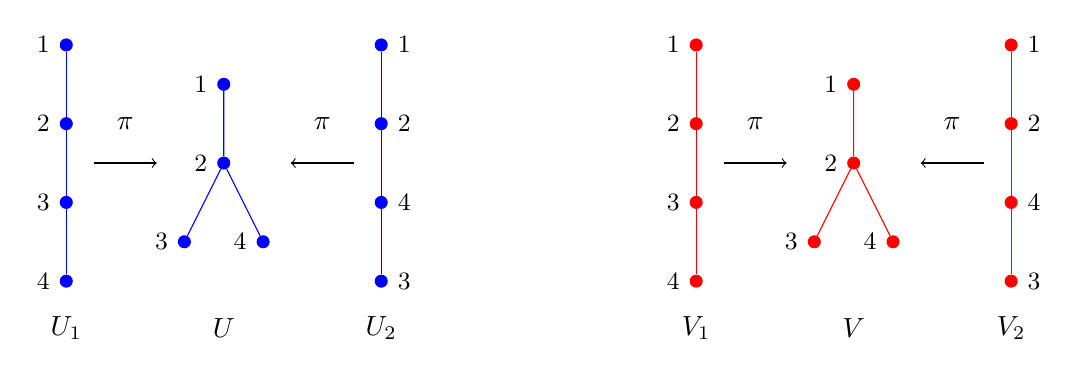
\begin{tikzpicture}
    \node[vertex,blue,fill=blue,label=right:{\small $1$}] at (5,3) (11) {};
    \node[vertex,blue,fill=blue,label=right:{\small $2$}] at (5,2) (12) {};
    \node[vertex,blue,fill=blue,label=right:{\small $4$}] at (5,1) (13) {};
    \node[vertex,blue,fill=blue,label=right:{\small $3$}] at (5,0) (14) {};
    \draw (11) [color=blue]--(12)--(13)--(14);
    \node at (5,-0.6)  (U2) {$U_2$};

    \node[vertex,,blue,fill=blue,label=left:{\small $1$}] at (1,3) (21) {};
    \node[vertex,,blue,fill=blue,label=left:{\small $2$}] at (1,2) (22) {};
    \node[vertex,,blue,fill=blue,label=left:{\small $3$}] at (1,1) (24) {};
    \node[vertex,,blue,fill=blue,label=left:{\small $4$}] at (1,0) (23) {};
    \draw (21) [color=blue]--(22)--(24)--(23);
    \node at (1,-0.6) (U1) {$U_1$};

    \draw[->] (4.65,1.5) -- (3.85,1.5);
    \node at (4.25,2) (pi) {$\pi$};
    \draw[->] (1.35,1.5) -- (2.15,1.5);
    \node at (1.75,2) (pi) {$\pi$};
    \node[vertex,blue,fill=blue,label=left:{\small $1$}] at (3,2.5) (31) {};
    \node[vertex,blue,fill=blue,label=left:{\small $2$}] at (3,1.5) (32) {};
    \node[vertex,blue,fill=blue,label=left:{\small $3$}] at (2.5,0.5) (33) {};
    \node[vertex,blue,fill=blue,label=left:{\small $4$}] at (3.5,0.5) (34) {};
    \draw (31)[color=blue]--(32)--(33);
    \draw (32)[color=blue]--(34);
    \node at (3,-0.6) (U) {$U$};

        \node[vertex,red,fill=red,label=right:{\small $1$}] at (13,3) (51) {};
    \node[vertex,red,fill=red,label=right:{\small $2$}] at (13,2) (52) {};
    \node[vertex,red,fill=red,label=right:{\small $4$}] at (13,1) (53) {};
    \node[vertex,red,fill=red,label=right:{\small $3$}] at (13,0) (54) {};
    \draw (51)[color=red]--(52)--(53)--(54);
    \node at (13,-0.6) (V2) {$V_2$};

    \node[vertex,red,fill=red,label=left:{\small $1$}] at (9,3) (41) {};
    \node[vertex,red,fill=red,label=left:{\small $2$}] at (9,2) (42) {};
    \node[vertex,red,fill=red,label=left:{\small $3$}] at (9,1) (44) {};
    \node[vertex,red,fill=red,label=left:{\small $4$}] at (9,0) (43) {};
    \draw (41)[color=red]--(42)--(44)--(43);
    \node at (9,-0.6) (V1) {$V_1$};

    \draw[->] (12.65,1.5) -- (11.85,1.5);
    \node at (12.25,2) (pi) {$\pi$};
    \draw[->] (9.35,1.5) -- (10.15,1.5);
    \node at (9.75,2) (pi) {$\pi$};
    \node[vertex,red,fill=red,label=left:{\small $1$}] at (11,2.5) (61) {};
    \node[vertex,red,fill=red,label=left:{\small $2$}] at (11,1.5) (62) {};
    \node[vertex,red,fill=red,label=left:{\small $3$}] at (10.5,0.5) (63) {};
    \node[vertex,red,fill=red,label=left:{\small $4$}] at (11.5,0.5) (64) {};
    \draw (61)[color=red]--(62)--(63);
    \draw (62)[color=red]--(64);
    \node at (11,-0.6) (V) {$V$};
    \end{tikzpicture}

\end{document}